\documentclass{article}

% Language and encoding
\usepackage[utf8]{inputenc}
\usepackage[english]{babel}

% Graphics
\usepackage{subfig}
\usepackage{graphicx}

% Mathematics and code
\usepackage{amsmath}
\usepackage{amsfonts}
\usepackage{listings}
\lstset{language=Python,keywordstyle={\bfseries \color{blue}}}

% References
\usepackage[style=numeric]{biblatex}
\addbibresource{bibliography.bib}

% Hyperlinks
\usepackage{xparse}
\usepackage[pdfborderstyle={/S/U/W 0}]{hyperref}
\urlstyle{same}

\begin{document}

\title{Linear classification of the IRIS dataset}
\author{Leik Lima-Eriksen and Torbjørn Bratvold}
\date{April 2020}

\maketitle
\begin{abstract}
    The choice of
 \end{abstract}
\newpage

\tableofcontents
\newpage

\section{Introduction}\label{sec:introduction}
The project described in this report has the goal of classifying samples of Iris flowers into
three different classes, namely the Setosa, Versicolor, and the Virginica. Classifying plants
based on their dimensions has multiple usages. For instance, it may be used by botanics as a tool
for easing their job. Also, it could be useful for mushroom enthusiasts to detect poisonous
mushrooms. And since classification algorithms may detect connections between classes and features
which may be hard for even the trained eye to spot, it could potentially outperform humans and
avoid disastrous misclassifications.

The Iris flowers have large (Sepal) and small (Petal) leaves, and the length and width of these
vary according to the class of flower. Thus, it seems natural to use those dimensions as features
for the classification. A dataset consisting of such measurements has been used in this project. 50
samples from each class has been provided. Their distributions are summarized in \autoref{fig:histograms}.

\begin{figure}[h]
    \centering
    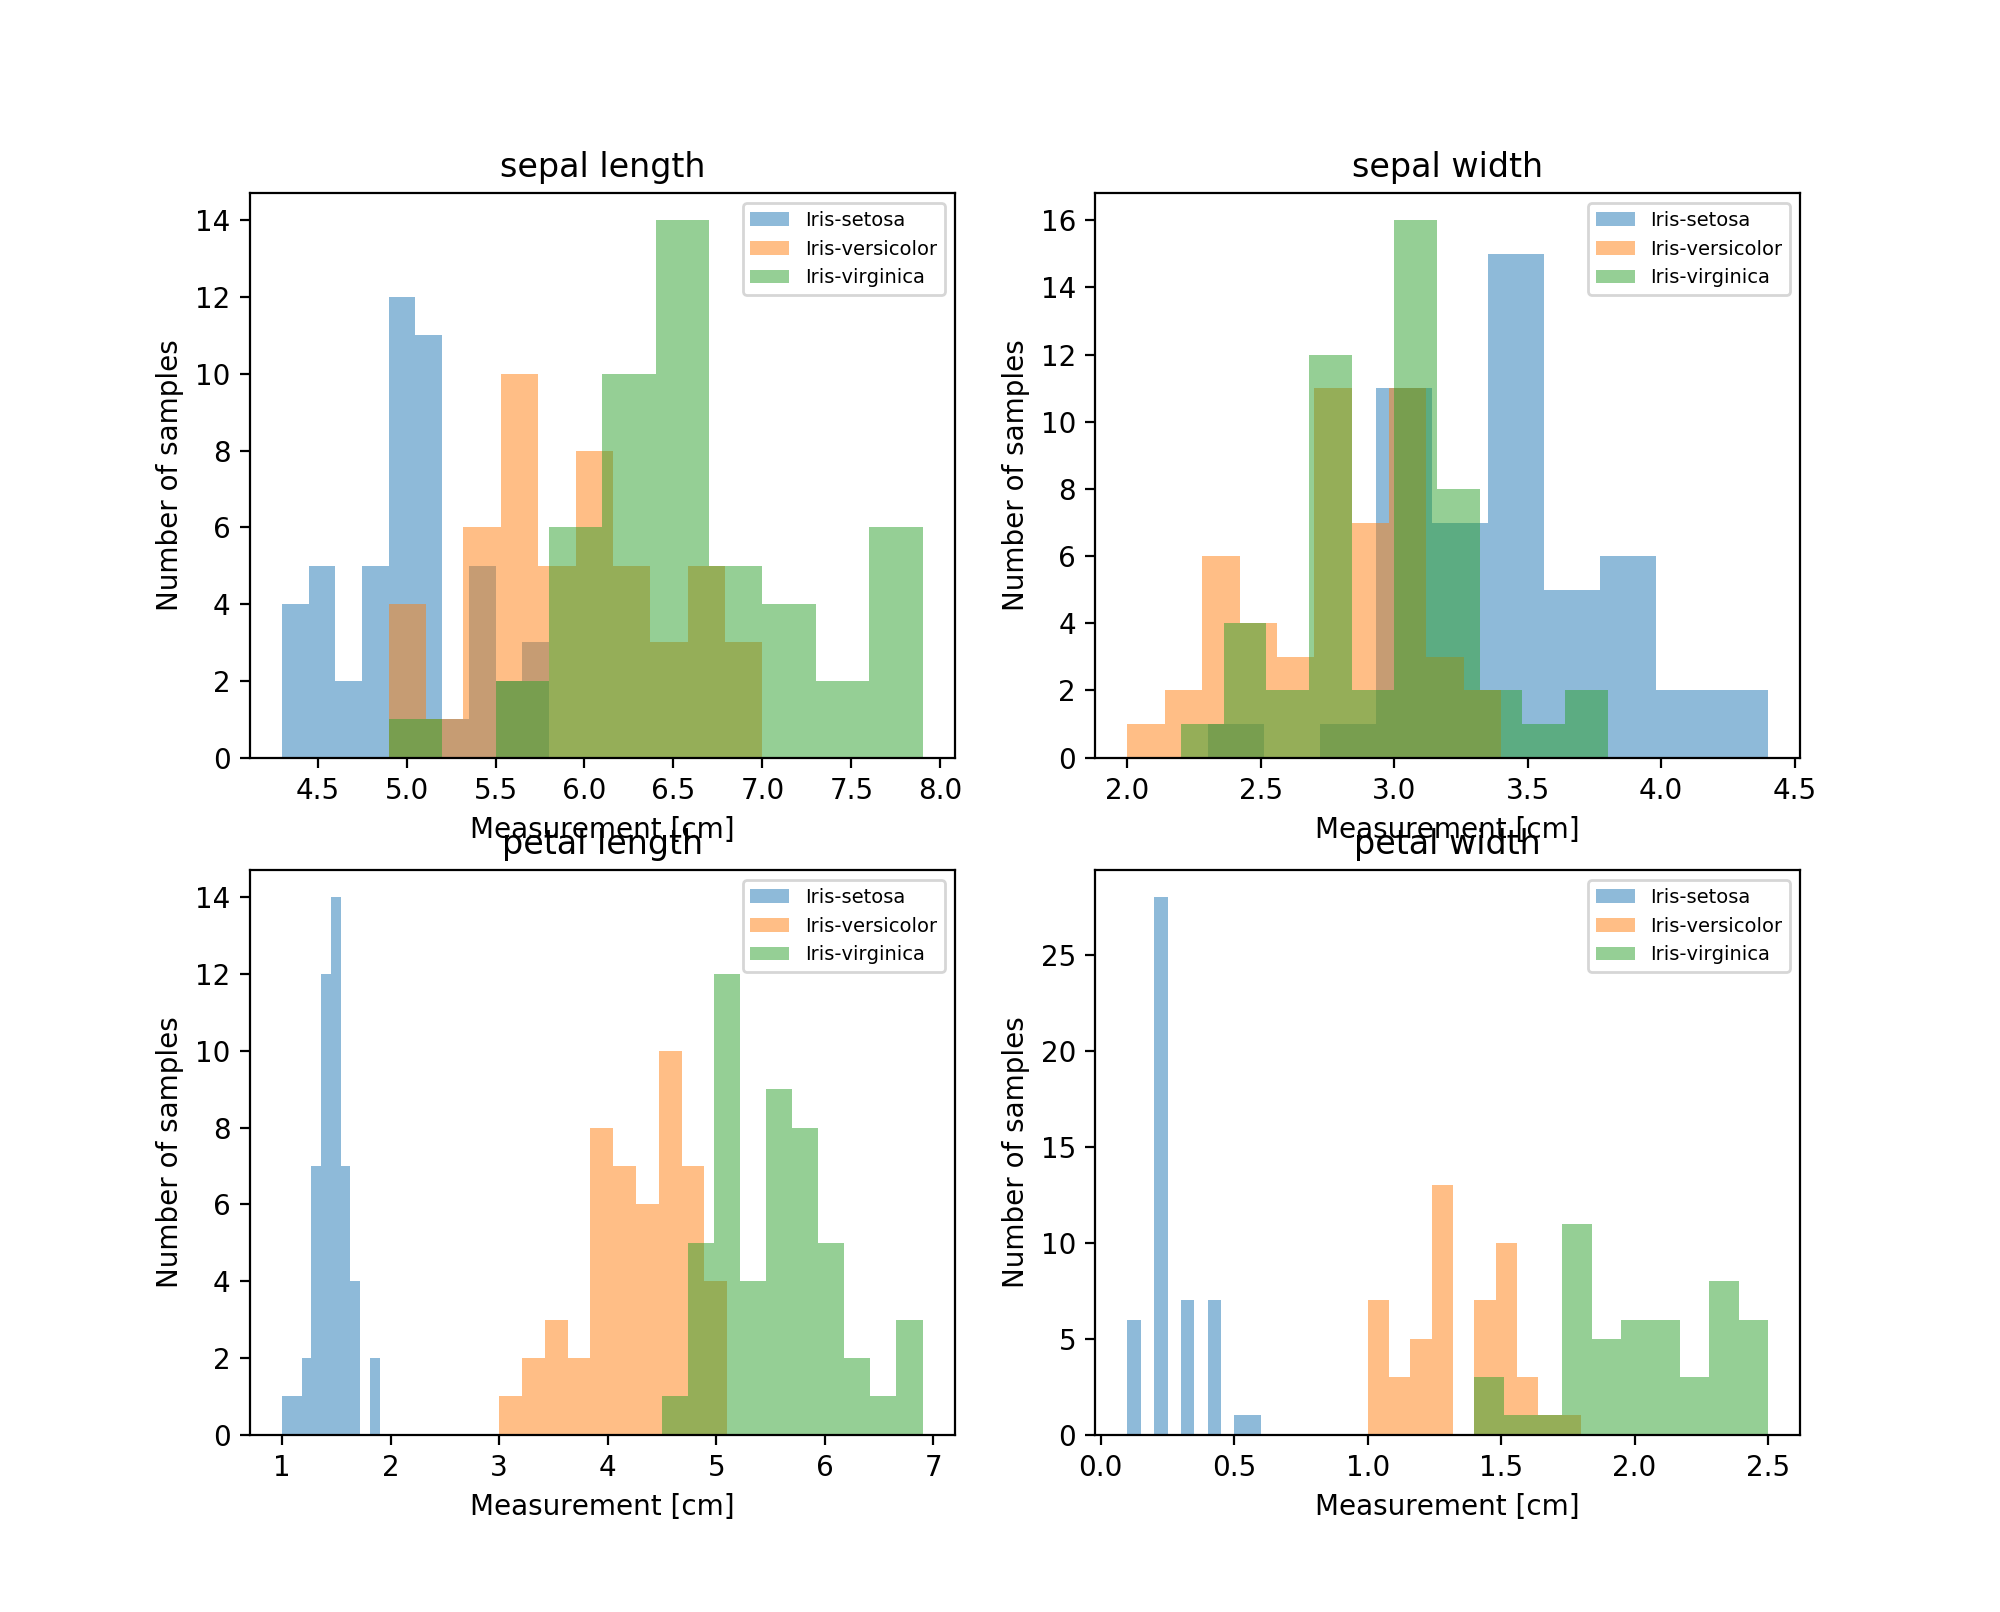
\includegraphics[width=0.9\textwidth]{../images/iris_histograms.png}
    \caption{Histograms for each of the attributes of the Iris flowers.}
    \label{fig:histograms}
\end{figure}

Observe that for the petal widths and lengths, the features are almost linearly separable, e.g.
there is little overlap in the measurements from each of the classes for these features. In contrast,
the sepal lengths and widths have quite large overlaps. Since two of the features are almost
linearly separable, a linear classifier will be used in this project.

\section{Theory}\label{sec:theory}

A linear classifier takes advantage of the fact that some classes may be separated by using a
linear operation on the dataset. Consider the scatter plot in \autoref{fig:petal_scatter_plot}.
Clearly, a line could be drawn in the middle of the void separating Iris Setosa samples from
Iris Versocolor samples. This line could then be used as a rule for classifying future samples
by just calculating which side of the line the new sample is on. It is not equally easy to
separate Versicolor from Virginica by using the same method - some of the Virginica samples overlap
with the Versicolor samples, and would then by misclassified. However, the error rate would be
quite small if the line is drawn in the middle of where the classes overlap. And in some cases,
such an error rate would be considered acceptable.

\begin{figure}
    \centering
    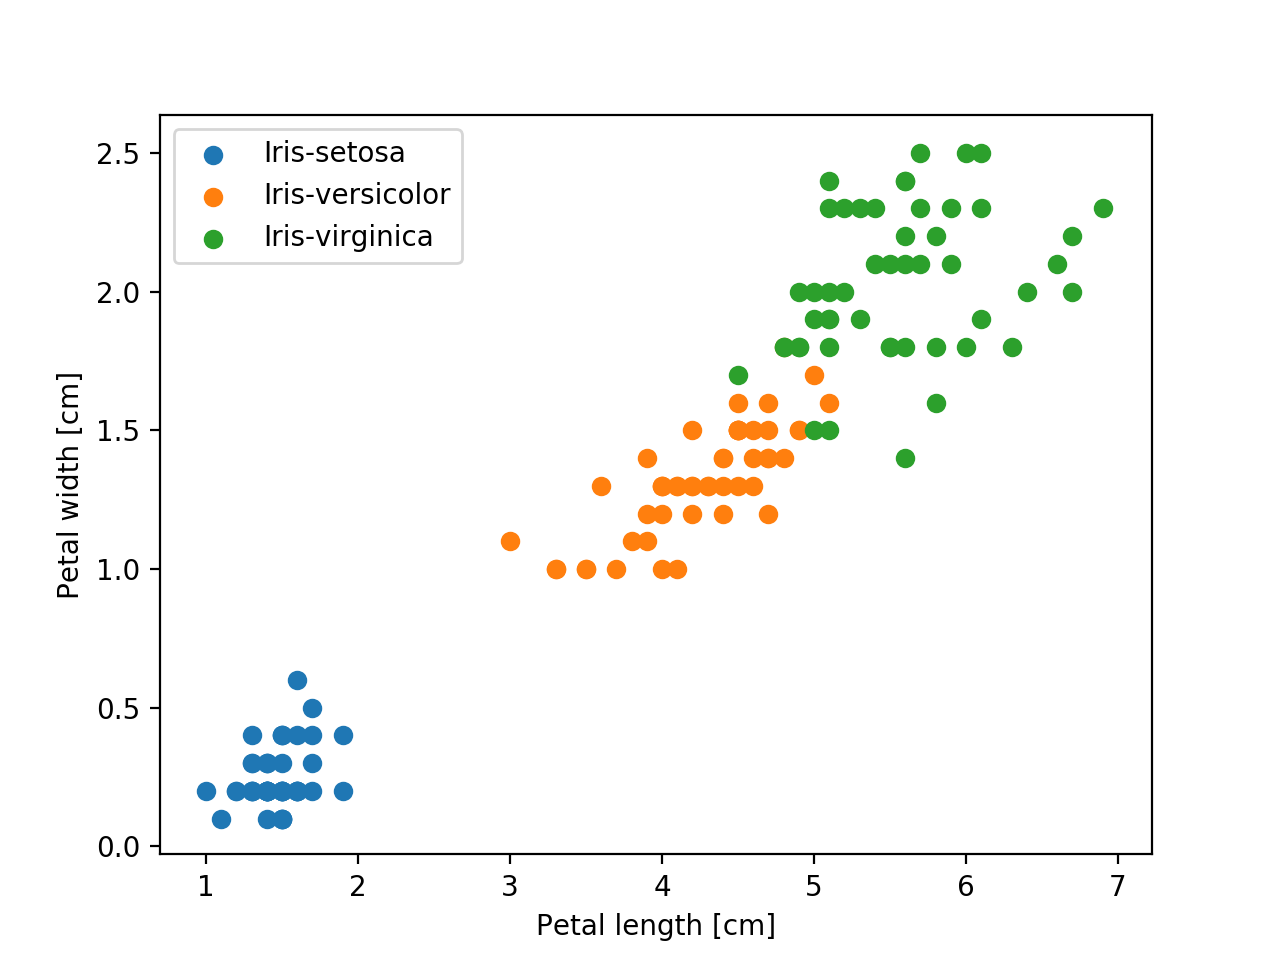
\includegraphics[width=0.8\textwidth]{../images/petal_scatter.png}
    \caption{Scatter plot for the Petal length and width of the Iris Setosa, Iris Versicolor,
    and Iris Virginica}
    \label{fig:petal_scatter_plot}
\end{figure}

In the case of the Iris dataset, there are four features to be considered. While a line of separation
in 2D translates to a plane in 3D, it would become a hyperplane in datasets with a feature dimension
$N > 3$.

Consider a dataset with $C > 2$ number of classes, and $D$ number of features. Since the goal of
a linear classifier is to construct hyperplanes of separation between samples of the classes,
these classes has to be represented numerically in some way (e.g., one cannot use a variable
with the value "Virginica" in a mathematical equation). Initially, one would think that
representing classes by distinct integers would be a good idea. However, this would imply
that the euclidian distance between two classes would be inherently greater than the distance
between two other classes. Intuitively, we know that this cannot be correct. To solve this problem,
we introduce a $\mathbb{R}^C$-space where each of the classes $c_i$ are represented by a vector $\vec{v_k}$ where

\begin{equation}
    v_{k,i} = \begin{cases}
        1 \enspace \forall \enspace i = k \\
        0 \enspace \forall \enspace i \neq k
    \end{cases} \enspace \forall \enspace j,k \in \{0, 1, 2, ..., C - 1\}\label{eq:class_vector}
\end{equation}

For instance, the class $c_2$ for a dataset with $C=3$ classes would be represented by
$\vec{v_2} = [ 0\enspace 1\enspace  0 ]^T$

Furthermore, we introduce the sample matrix $x$, which holds the measurements of the features from
all of the labeled samples. Let $N$ be the number of samples available in the dataset. Also,
let $x_k = \{m_j\} \enspace \forall \enspace j \enspace \in \{0, 1, 2, ..., D - 1\}$ be a sample vector containing
the measurements $m_j$ from each of the features of the k-th sample. Then $x = \{x_k\} \enspace \forall \enspace k \enspace
\in \{0, 1, 2, ..., D - 1\}$. The matrix $t = \{t_k\} \enspace \forall \enspace k \enspace
\in \{0, 1, 2, ..., D - 1\}$ should contain the vector representation of the true label for each of the samples
$x_k$ in the same order. We also need to add a 1 as the last element of the sample vectors such that
$[ x^T \enspace 1 ^T ] \rightarrow x$. This is done so that the further calculations can include constants.

If the dataset is linearly separable, then there exists a weighing matrix $W$ of dimensions $C \times (D+1)$ such
that
\begin{equation}
    z_k = Wx_k \label{eq:z_k}
\end{equation}
reveals a continuous vector representation of how likely it is for a sample $x_k$ to belong to the class
$c_i$ in the relation $i = argmax(u(z_k))$, where $u$ is the elementwise heaviside function. Then one could
easily classify a future sample $x_{N+1}$ just by using \eqref{eq:z_k}.

For the most cases, however, $g_k \neq t_k $ for all samples $x_k$ since the samples are not linearly
separable. Such a case is depicted in \autoref{fig:squashing_functions}. The heaviside score function is referenced
as $u(x)$. Clearly, $u(x)$ will misclassify the $c_1$ sample with value $1$ as a $c_2$ sample. Since
we in our case have several features of interest, this squashing function would lead us to an output
where our classifier will classify some samples as belonging to two classes. It would be more
correct to give measurements close to the separation line a score more in the middle of the two classes,
such that our classifier will not take such scores equally into consideration as measurements where
the value clearly belongs to one specific score.

\begin{figure}
    \centering
    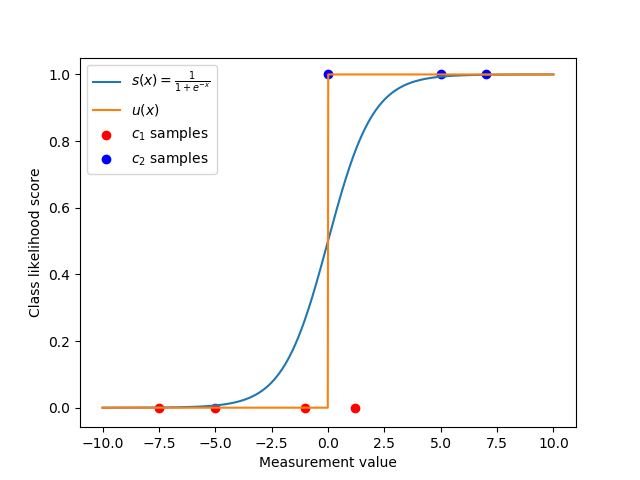
\includegraphics[width=0.8\textwidth]{../images/squashing_functions.png}
    \caption{Comparison of the class likelihood score for different types of squashing functions.}
    \label{fig:squashing_functions}
\end{figure}

One such function is the sigmoid function described by \eqref{eq:sigmoid}. By inserting \eqref{eq:z_k}
into \eqref{eq:sigmoid}, we get a good score function $g_k$ as in \eqref{eq:score_function}
which can classify samples.

\begin{equation}
    s(x) = \frac{1}{1 + e^{-x}} \label{eq:sigmoid}
\end{equation}

\begin{equation}
    g_k = \frac{1}{1 + e^{-Wx_k}} \label{eq:score_function}
\end{equation}

For a future sample $x_{N+i}$ one would then classify it as the class $c_i$ of minimum euclidian
distance between $v_i$ and $g_k$.

The next step in developing the linear classifier is to train it on our dataset.
The linear classifier is not statisctically based, and so one could not use an optimization
criterion such as ML for calculating $W$. Instead, a quite popular variant is the Mean Square
Error (MSE) optimization. The $MSE$ of the linear classifier is given in \eqref{eq:MSE}.

\begin{equation}
    \textnormal{MSE} = \frac{1}{2} \sum_{k=0}^{N-1} (g_k - t_k)^T(g_k - t_k) \label{eq:MSE}
\end{equation}

The minimization of MSE would lead to the value of $W$ which on average gives the smallest error
between its predicted labels $g_k$ and the corresponding true labels $t_k$. Since it is a sum of
squares of the errors, it penalizes large deviations much more than small deviations.

Since there exists no explicit solution to finding the minimum of the MSE with respect to W,
we have to reside to a gradient based technique. In essence, we will through iterations calculate
the $\nabla_W MSE$, and update $W$ in the opposite direction of the gradient with a
small step factor $\alpha$.

\begin{equation}
    W(m) = W(m-1) - \alpha \nabla_W\textnormal{MSE} \label{eq:W_iteration}
\end{equation}

The gradient of the MSE can easily be found by using the chain rule for gradients. Then we get the
relation \eqref{eq:grad_W_MSE}.

\begin{equation}
    \nabla_WMSE = \sum_{k=0}^{N-1} \nabla_{g_k} MSE \nabla_{z_k} g_k \nabla_W z_k \label{eq:grad_W_MSE}
\end{equation}
where
\begin{align*}
    \nabla_{g_{k}} M S E &=g_{k}-t_{k} \\
    \nabla_{z_{k}} g &=g_{k} \circ\left(1-g_{k}\right) \\
    \nabla_{W} z_{k} &=x_{k}^{T}
\end{align*}

It is customary to initialize $W(0) = 0$. The step factor $\alpha$ should then be tuned to fit the dataset.
A too great value will result in oscillations of $W$ around its minimum whereas a too low value will
require a lot more iterations than necessary. Lastly, the number of iterations has to be chosen.
A larger number of iterations is always better, but after a certain number of iterations we will
not gain a better $W$. So this number should just be "great enough".

\section{Goals}\label{sec:purpose}

The purpose of this project is to design a linear classifier for the Iris dataset,
and explore how varying the training set and features affects the performance of
this classifier. We will first train the classifier by using all features, and tune
the step factor $\alpha$. The performance will be evaluated in terms of the error
rate and the confusion matrix. Then we will choose different samples for training,
and compare the performance of the two training sets.

In the last part, we will take a closer look at how linear separability of features
affects the performance of the classifier. More specifically, we will exclude the
least linearly separable features from the dataset one at a time and evaluate the
performance.

\section{Implementation and results}\label{sec:implementation_and_results}

The linear classifier has been implemented in Python3.6. Numpy was used for
representing vectors and matrices as it provides powerful methods for applying
linear algebra in a fast and easy-to-read manner. For plotting, we chose to stick
with the well-renowned plotting library Matplotlib. This library has several
handy features for plotting all relevant kinds of figure used in this project.

The Iris dataset contains three different classes. The vector representation used
in our implementation is listed in \autoref{tab:class_vectors}, but it should be
said that the mapping is trivial for the performance of the classifier.

\begin{figure}
    \centering
    \begin{tabular}{ | c | c | }
        \hline
        Class name $c_i$ & Vector representation $v_i$ \\
        \hline
        Iris Setosa & $[1 \enspace 0 \enspace 0]^T$ \\
        Iris Versicolor & $[0 \enspace 1 \enspace 0]^T$ \\
        Iris Virginica & $[0 \enspace 0 \enspace 1]^T$ \\
        \hline
    \end{tabular}
    \caption{trololo}
    \label{tab:class_vectors}
\end{figure}

The dataset is imported from a CSV file where each row represents a sample. The first four columns
represents the measurements of the different features, whereas the last columnn specifies the label of
the sample, e.g. which class it belongs to.

\begin{figure}
    \centering
    \begin{tabular}{ | c | c | }
        \hline
        Index & Meaning \\
        \hline
        0 & Sepal length \\
        1 & Sepal width \\
        2 & Petal length \\
        3 & Petal width \\
        (4) & Label \\
        \hline
    \end{tabular}
    \caption{Overview of the meaning of each column in the dataset CSV file.}
    \label{tab:class_vectors}
\end{figure}

The function \lstinline{load_dataset} is first used to load the dataset from file into memory.
Two arrays - \lstinline{samples} and \lstinline{labels} - are returned, where the true label of
\lstinline{samples[i]} is \lstinline{labels[i]}. This dataset is further divided into a training
dataset and a test  dataset by using the function \lstinline{split_dataset(samples, labels, split_index)},
where \lstinline{split_index} indicates how many samples of each class should belong to the training
data set.

As described in \autoref{sec:theory}, all samples first have to be extended with a 1 as their last element.
Thereafter, we need to convert the labels from their original string representation to a vector
representation by the rule of \eqref{eq:class_vector}. This is done element-wise on the string labels by
using the \lstinline{label_string_to_vector} function.

The extended training samples together with the labels on vector form is fed into the implementation of
a linear classifier called \lstinline{train_linear_classifier}. This function calculates the weighing matrix
$W$ as described in \eqref{eq:W_iteration} using a total of \lstinline{num_iterations} number of iterations
with an $\alpha$ described by its parameter \lstinline{alpha}. Also, for each iteration the current weighing
matrix $W(m)$ is used on the test set to predict the labels of the test samples using
\lstinline{get_predicted_label_vectors}. These label vectors are then compared against the true
label vectors and the MSE for this iteration is calculated using \eqref{eq:MSE}, which is implemented
in \lstinline{get_MSE}. In addition, we use the \lstinline{get_error_rate} on these label vectors
to calculate the ratio of misclassified samples per iteration.

It was mentioned in \autoref{sec:theory} that $\alpha$ should be tuned such that the MSE neither
oscillates (too high $\alpha$) nor does not converge (too low $\alpha$). In order to visualize
how the choice of different $\alpha$s affect the $MSE$s as a function of the number of iterations,
such a function has been plotted for $\alpha \enskip \in \enskip \{0.0025, 0.005, 0.0075, 0.01\}$
in \autoref{fig:MSE_alphas_30_first} by using the function called \lstinline{plot_MSEs}.

\begin{figure}
    \centering
    \subfloat[MSE]{%
      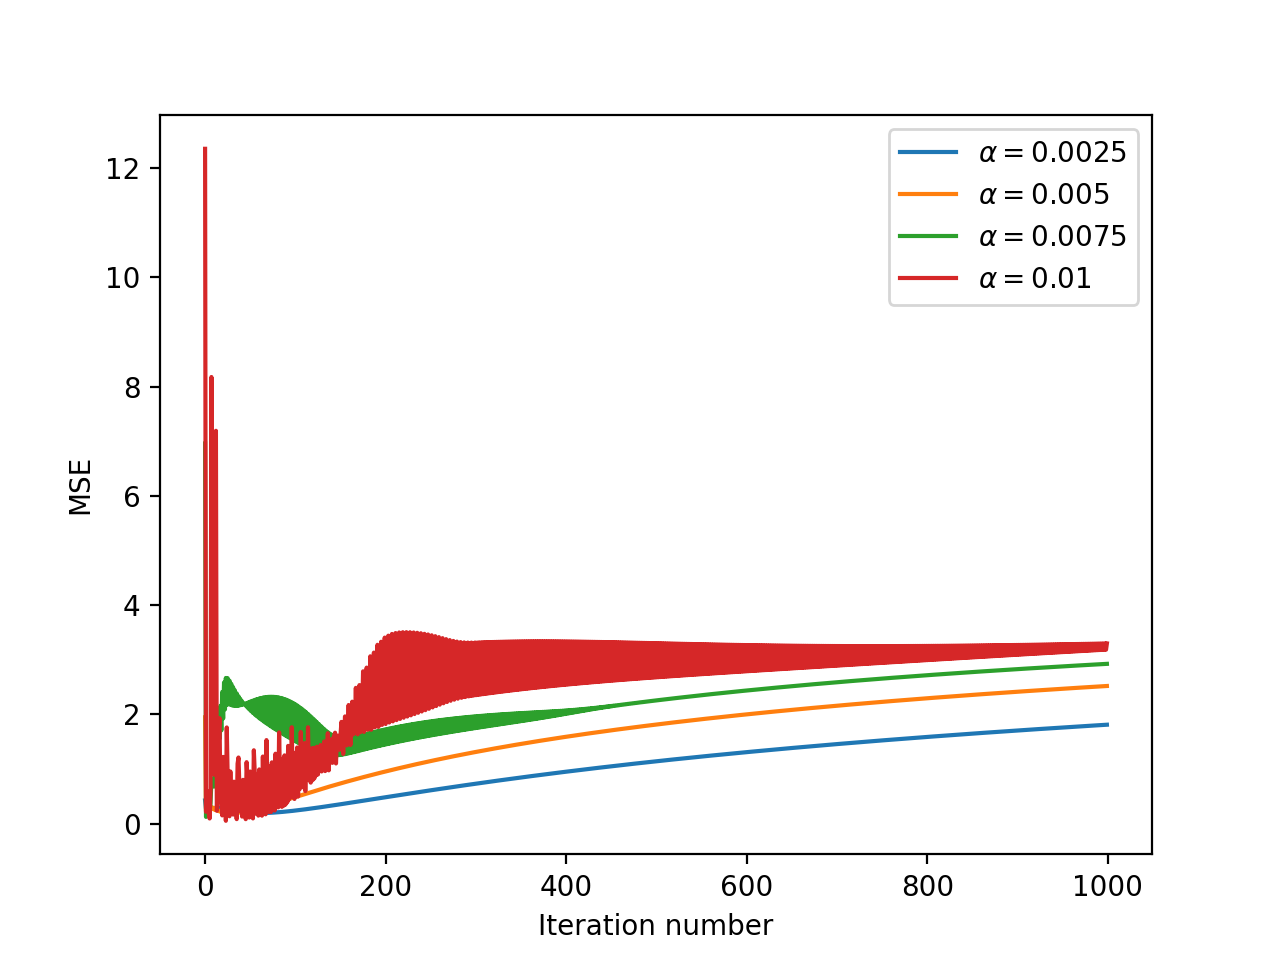
\includegraphics[width=0.55\textwidth]{../images/MSE_alphas_30_first.png}%
      \label{fig:MSE_alphas_30_first}%
    }
    \subfloat[Error rate for $\alpha=0.005$]{%
      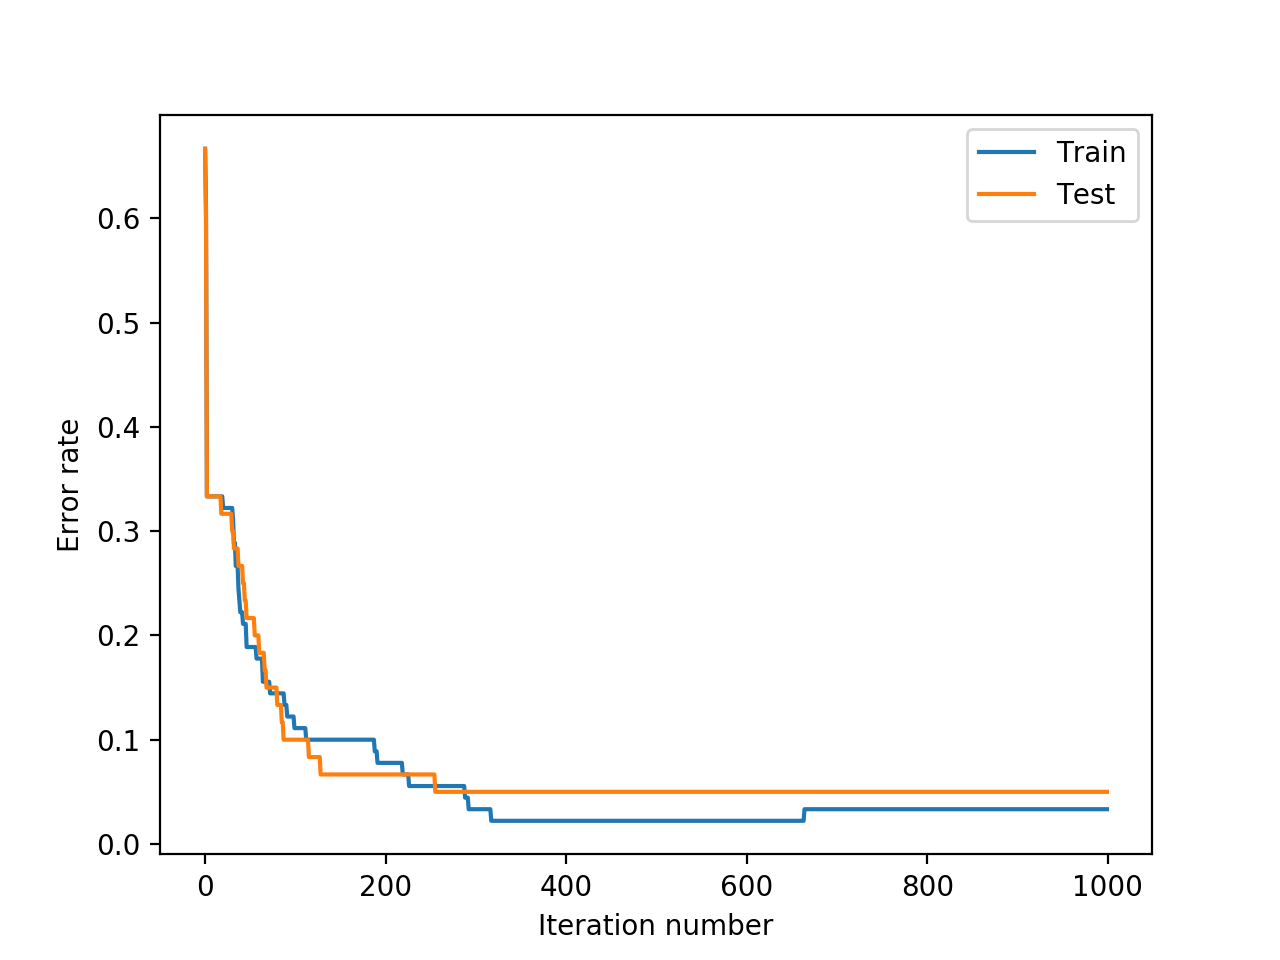
\includegraphics[width=0.45\textwidth]{../images/error_rate_30_first.png}%
      \label{fig:error_rate_30_first}%
    }
    \caption{Mean Square Error (MSE) and error rate as a function of the number of iterations on W
    for different values of $\alpha$. Using 30 first samples for training}
\end{figure}

Clearly, one can see that an $\alpha \geq 0.0075$ makes the MSE oscillate as a function of the number
of iterations. This is an indication of that \eqref{eq:W_iteration} makes the MSE overshoot its
minimum value instead of monotonically approaching it. And for $\alpha \leq 0.0025$ it converges
too slowly. Thus $\alpha = 0.005$ seems to be the sweet spot, and so is the value which will be used
for this partitioning of the dataset.

One further has to decide on the number of iterations necessary for the training to converge. This
is impossible to estimate from \autoref{fig:MSE_alphas_30_first}. In order to find this out,
we have to plot the error rate as a function of the number of iterations. This has been done in
\autoref{fig:error_rate_30_first} by using the function \lstinline{plot_error_rates}. By reading the graph,
the error rate seems to stop decending after $\approx 300$ iterations. It is worth noting that the true error rate
actually continues to decend, but since we have a discrete number of test samples, the discrete error rate
can only decrement by a discrete number of samples and so would not be able to decrease any further.
This may prove different for larger datasets, but either way the increase in performance would only be
marginal.

With these values, we get an error rate of $5\%$ the test set and $3.33\%$ on the training set. This
also seems to be quite reasonable for a linear classifier: By inspecting \autoref{fig:petal_scatter_plot},
we observe that $\approx 5$ out of 50 samples are not linearly separable by their Petal dimensions.
In order to gain further insights into which samples where misclassified, a confusion matrix comes in
handy. Such a matrix has the different true labels listed along the columns and the predicted labels
along the columns. Each cell then gives the number of samples of a certain true label was classified
as a particular predicted label. The confusion matrices for both the test set and the training set are
plotted in \autoref{fig:CM_30_first}. We see that a trend is that samples of Versicolor get classified
as Virginica. This is in compliance with \autoref{fig:histograms}, where we see that samples of
those classes are the most overlapping.

\begin{figure}
    \centering
    \subfloat[Test dataset]{%
      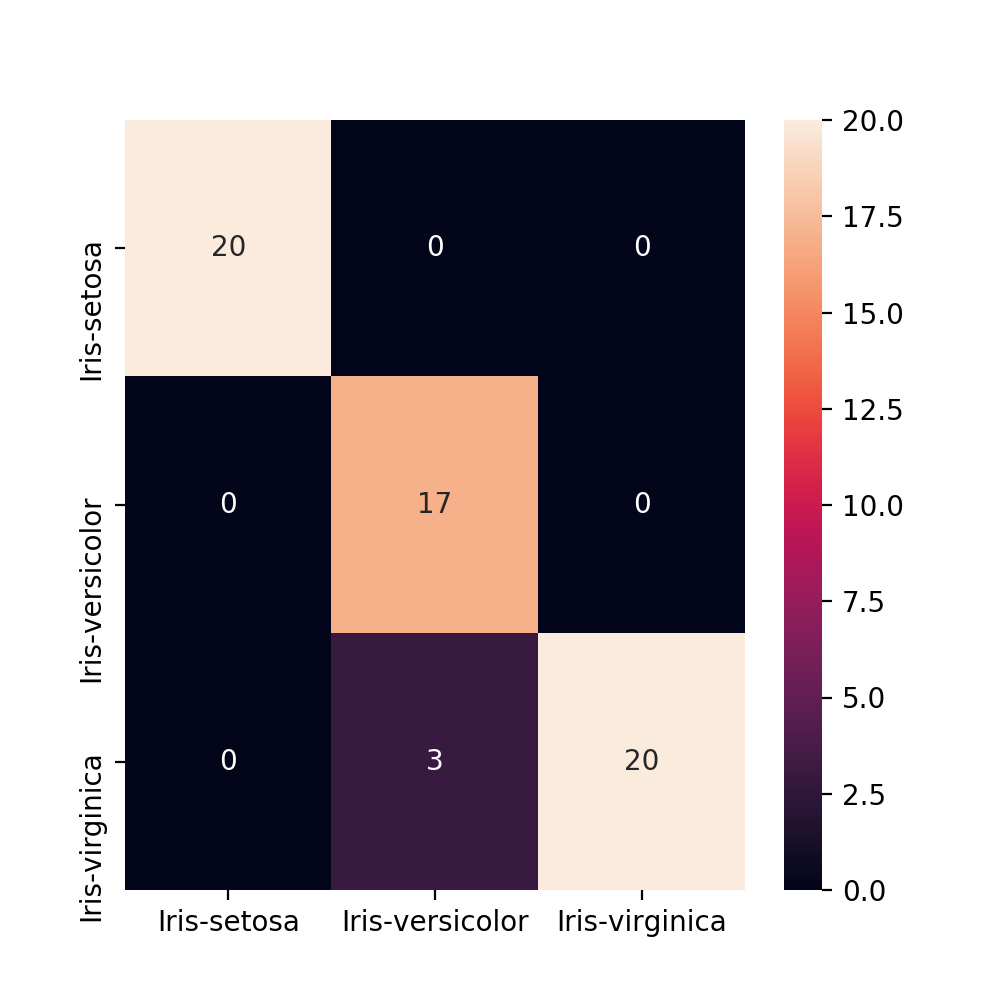
\includegraphics[width=0.45\textwidth]{../images/CM_test_30_first.png}%
      \label{fig:CM_test_30_first}%
    }\qquad
    \subfloat[Train dataset]{%
      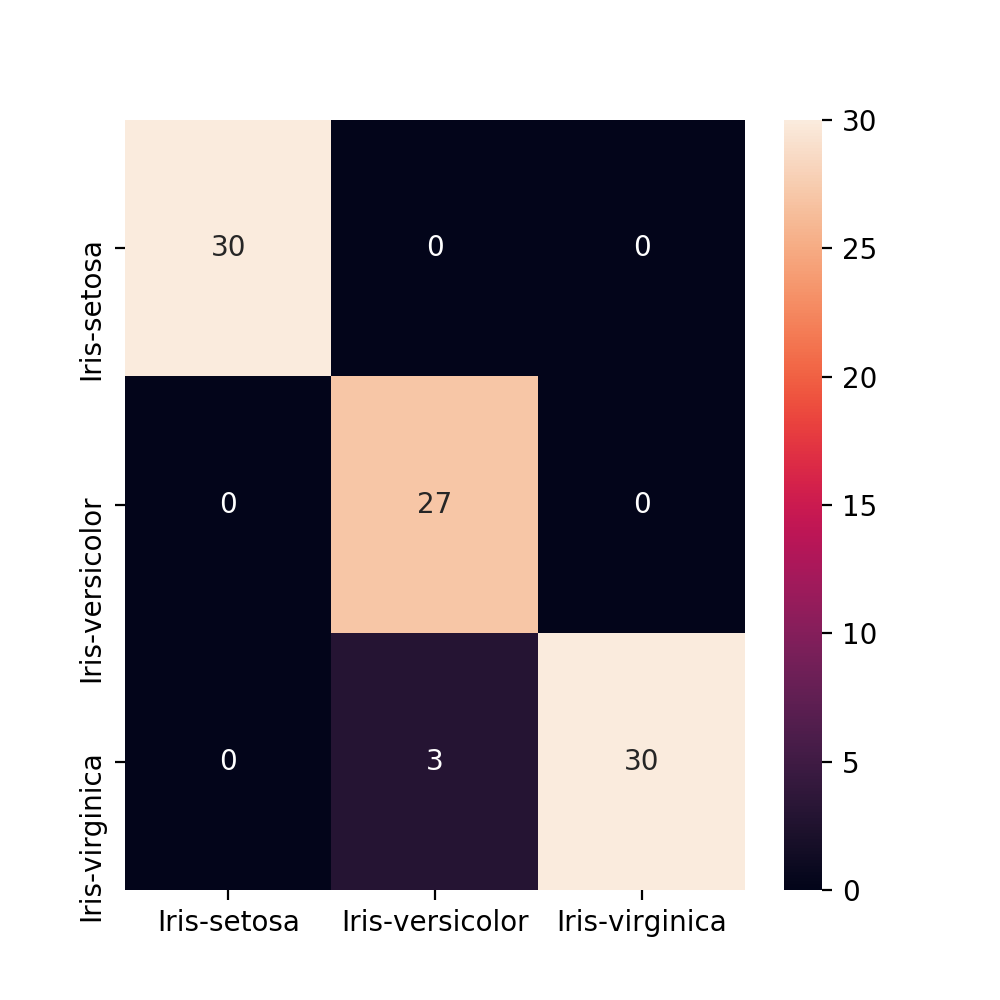
\includegraphics[width=0.45\textwidth]{../images/CM_train_30_first.png}%
      \label{fig:CM_train_30_first}%
    }
    \caption{Confusion matrices gained by using the first 30 samples as train dataset;%
    $\alpha = 0.005$; 300 iterations on $W$.}\label{fig:CM_30_first}
\end{figure}

Now we turn our attention into researching how the choice of train samples affect the performance of
the classifier. Instead of using the first 30 samples for training, we will use the last 30 samples.
The same procedure for tuning $\alpha$ and number of iterations is used on this new partitioning.
$MSE$ does not seem to converge earlier in \autoref{fig:MSE_alphas_30_last}, and so
$\alpha = 0.005$ is used. By inspecting the error rate in \autoref{fig:error_rate_30_last}, we observe that we
need to use 400 iterations in order for the error rate to approach its minimum. This results in an error rate of
$1.6\%$ for the test set and $5.5\%$ for the training set.

\begin{figure}
    \centering
    \subfloat[MSE]{%
      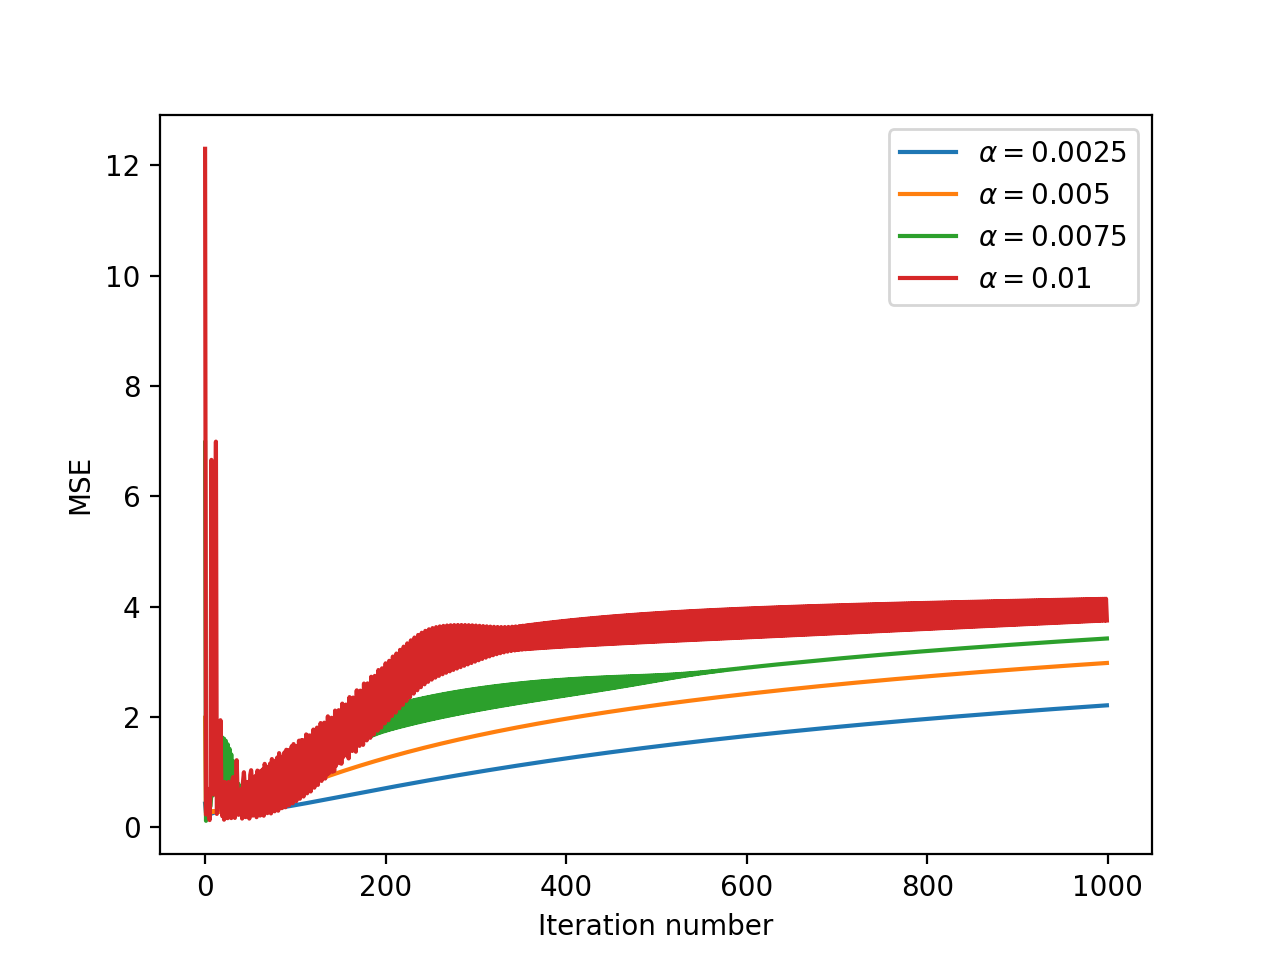
\includegraphics[width=0.55\textwidth]{../images/MSE_alphas_30_last.png}%
      \label{fig:MSE_alphas_30_last}%
    }
    \subfloat[Error rate for $\alpha=0.005$]{%
      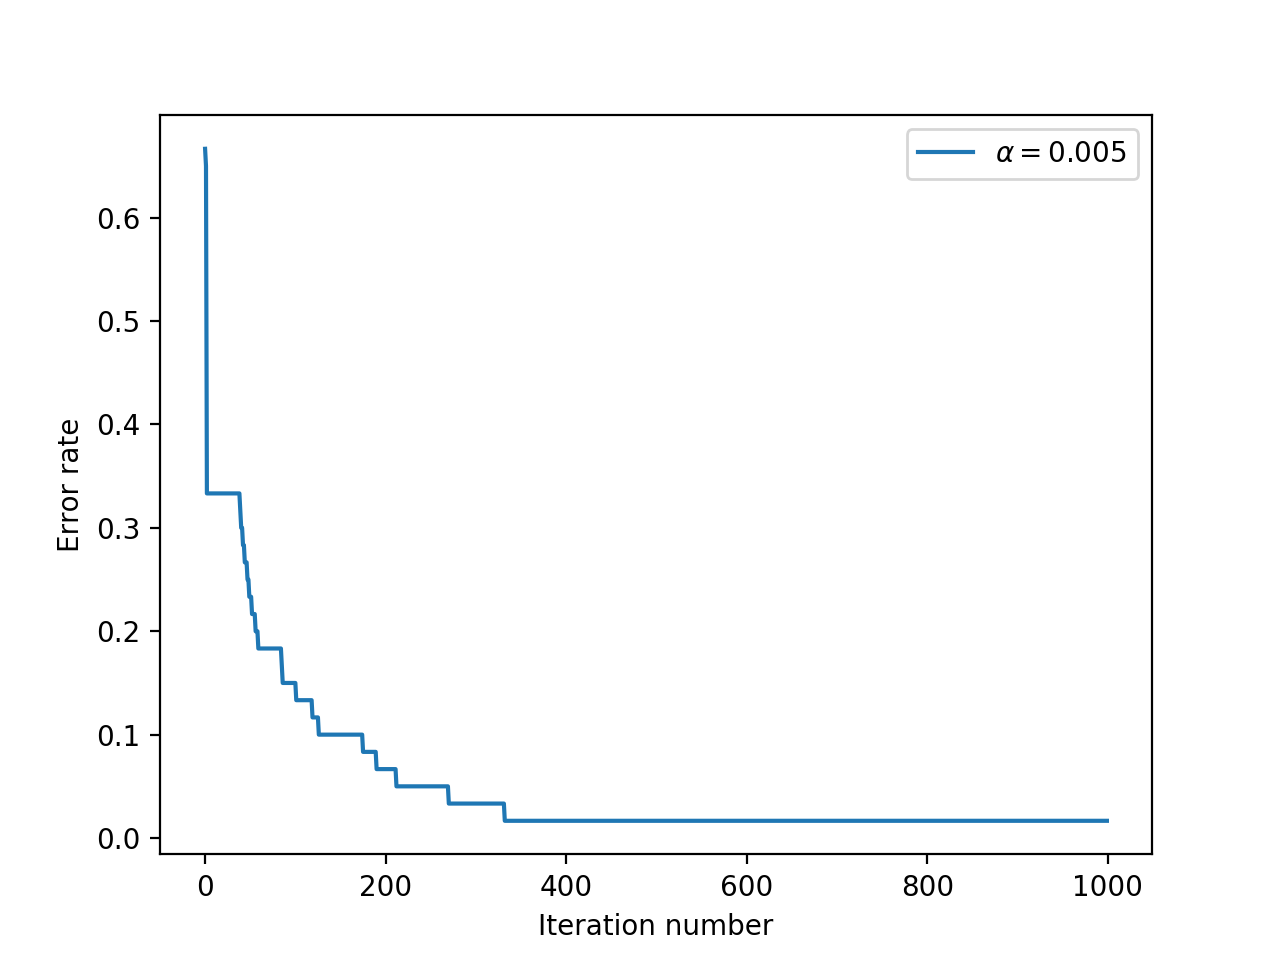
\includegraphics[width=0.45\textwidth]{../images/error_rate_30_last.png}%
      \label{fig:error_rate_30_last}%
    }
    \caption{Mean Square Error (MSE) and error rate as a function of the number of iterations on W
    for different values of $\alpha$. Using 30 last samples for training.}
\end{figure}

It may at first seem reasonable that this linear classifier performs better with the last 30 samples for training
since it  has a much lower error rate on the test set. However, as the cofusion matrices in \autoref{fig:CM_30_last}
reveals, it actually has just a similar performance - the classifier misclassifies in total 6 Versicolors as
Virginica. So in this case, the choice of training samples has no impact on the overall performance of the
classifier.

\begin{figure}
    \centering
    \subfloat[Test dataset]{%
      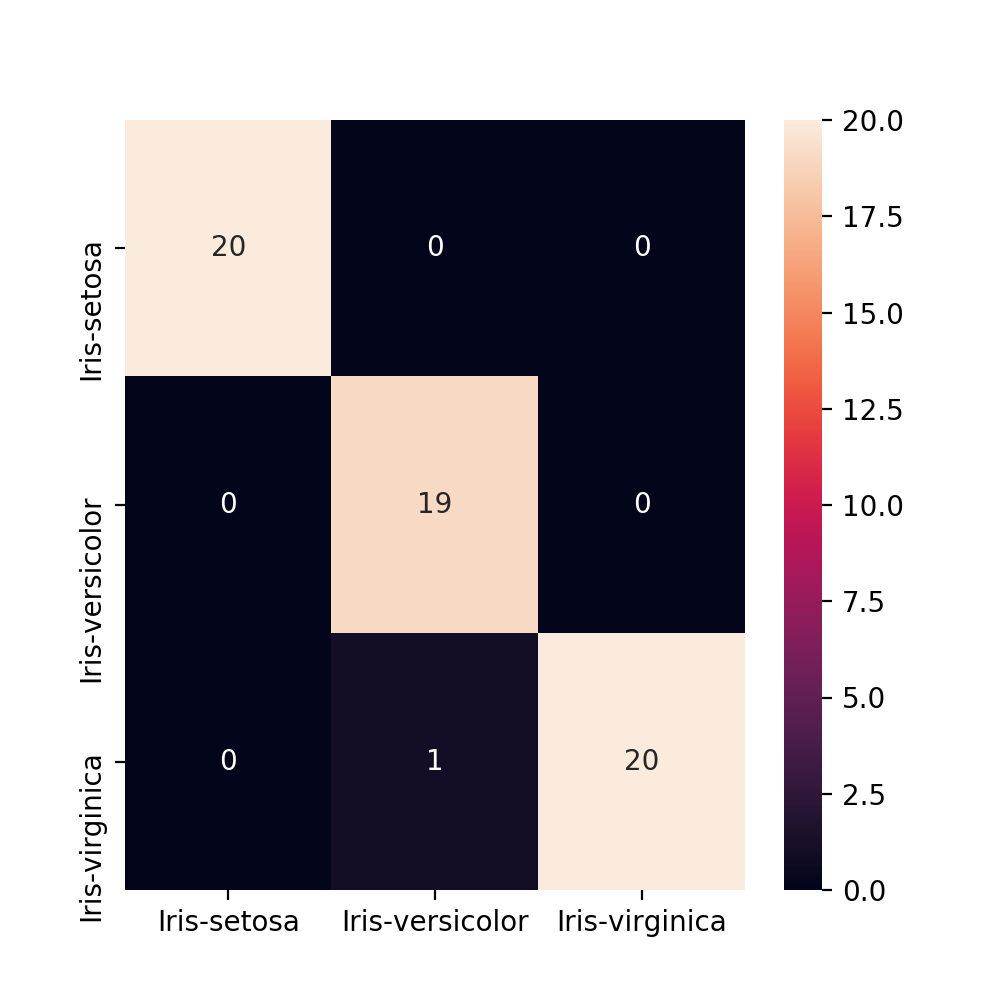
\includegraphics[width=0.45\textwidth]{../images/CM_test_30_last.png}%
      \label{fig:CM_test_30_last}%
    }\qquad
    \subfloat[Train dataset]{%
      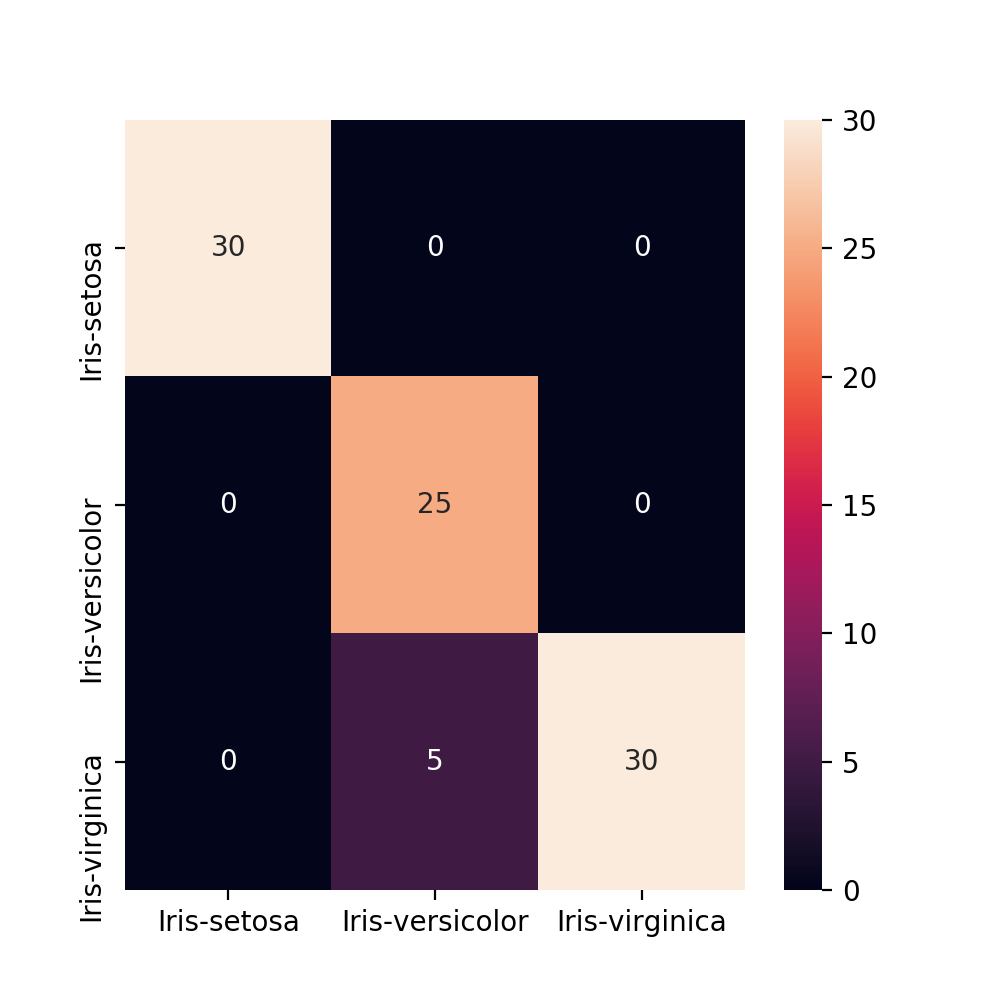
\includegraphics[width=0.45\textwidth]{../images/CM_train_30_last.png}%
      \label{fig:CM_train_30_last}%
    }
    \caption{Confusion matrices gained by using the last 30 samples as train dataset;%
    $\alpha = 0.005$; 400 iterations on $W$.}\label{fig:CM_30_last}
\end{figure}

From \autoref{sec:introduction} we saw how Sepal width and Sepal length was the two features which overlapped
the most in measurements, meaning they were the least linearly separable. By inspecting \autoref{fig:histograms},
we see that the most overlap occurs for the Sepal width. Thus it would be interesting to see how a linear classifier would
perform on the dataset with the Sepal width feature removed.

MSE as a function of number of iterations on $W$ has been plotted in \autoref{fig:MSE_no_sepal_width},
and we see that we now require a slightly higher $\alpha=0.006$. But what turns out to be different,
is that the error rate now converges more slowly, as shown in \autoref{fig:error_rate_no_sepal_width}.
One would initially think that a higher $\alpha$ makes the $MSE$ converge faster. However it turns
out that the $\nabla MSE$ is actually smaller without this feature, and thus it requires $1000$
iterations inn order for it to converge. This can in some way be explained by inspecting
\autoref{fig:histograms}; since the measurements have a small variance in Sepal width,
this feature will contribute to a larger partial derivative and thus make the MSE converge faster.


\begin{figure}
    \centering
    \subfloat[MSE]{%
      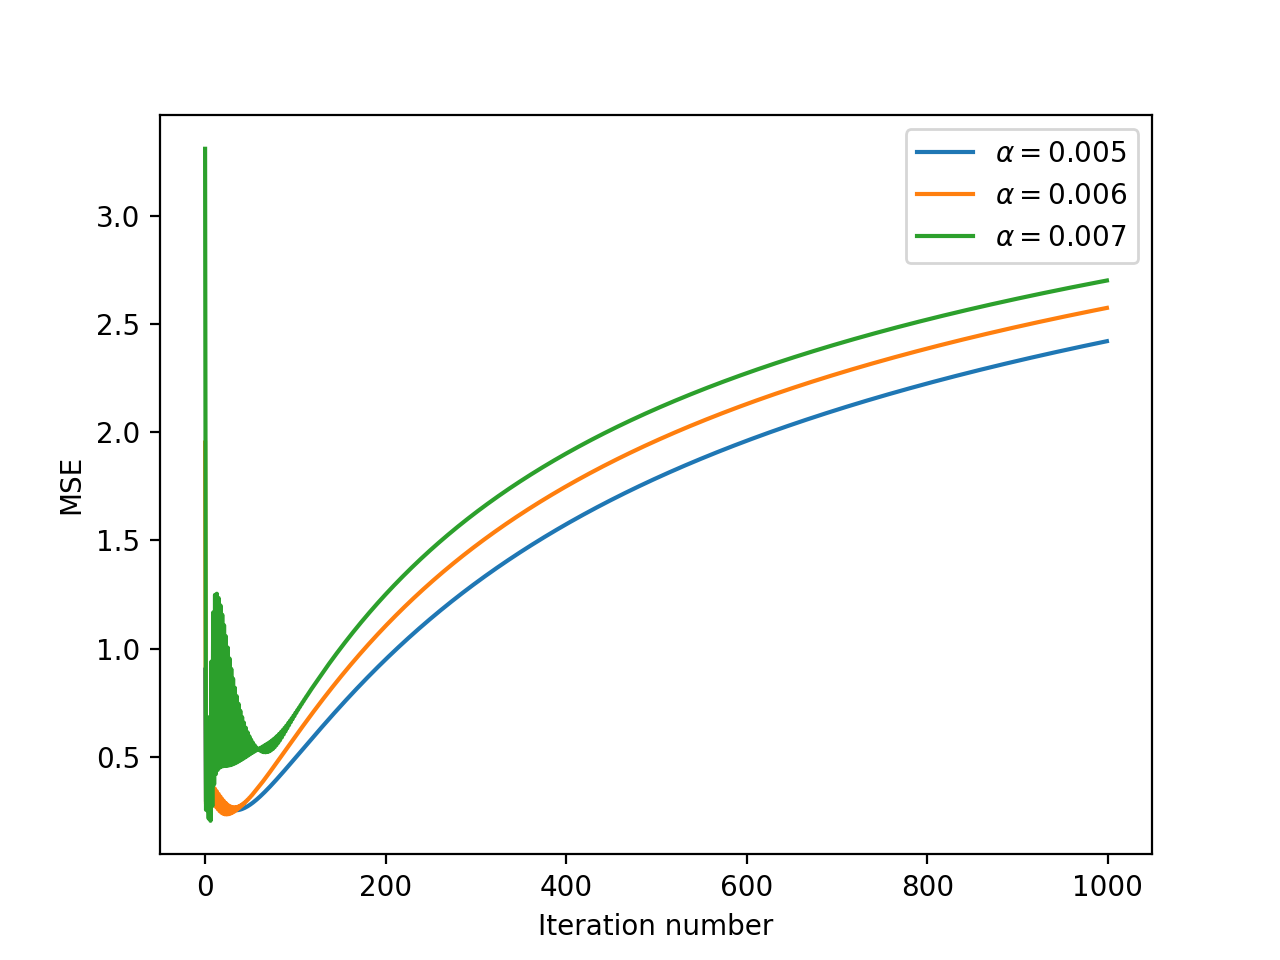
\includegraphics[width=0.55\textwidth]{../images/MSE_no_sepal_width.png}%
      \label{fig:MSE_no_sepal_width}%
    }
    \subfloat[Error rate for $\alpha=0.006$]{%
      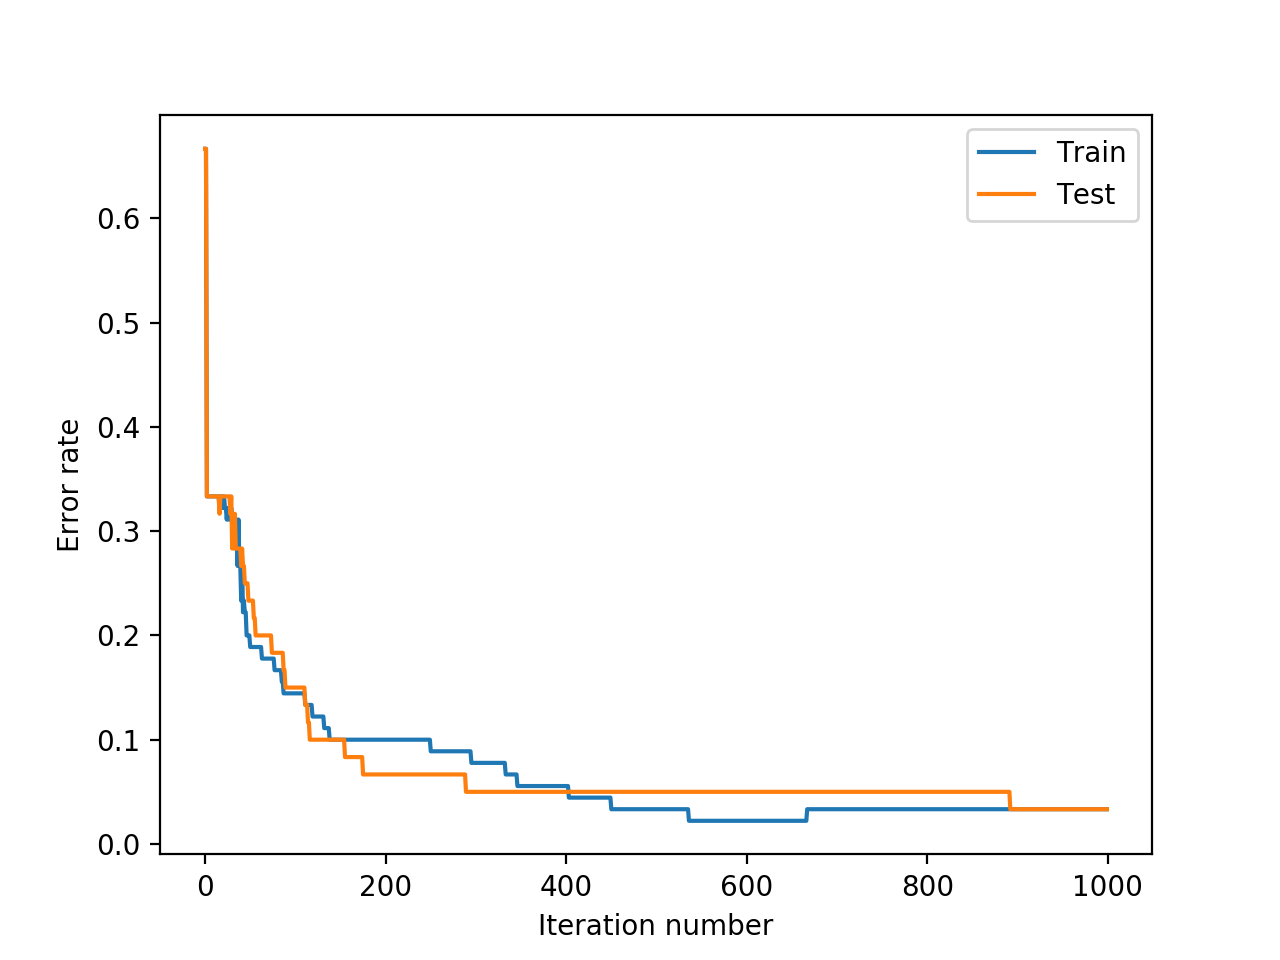
\includegraphics[width=0.45\textwidth]{../images/error_rate_no_sepal_width.png}%
      \label{fig:error_rate_no_sepal_width}%
    }
    \caption{Mean Square Error (MSE) and error rate as a function of the number of iterations on W
    for different values of $\alpha$. Using dataset without Sepal width.}
\end{figure}

Inspecting the confusion matrices in \autoref{fig:CM_no_sepal_width}, we immidiately see that
the classifier reveals fewer misclassifications on the dataset as a whole - we now get only
5 misclassified flowers instead of our previous 6 misclassifications. The error rate for both
the test dataset and the training dataset was found to be $3.33\%$. This lower error is also
something that we could have expected - we have now removed a feature which was not linearly
separable at all, and only contributed to mixing in errors.

\begin{figure}
    \centering
    \subfloat[Test dataset]{%
      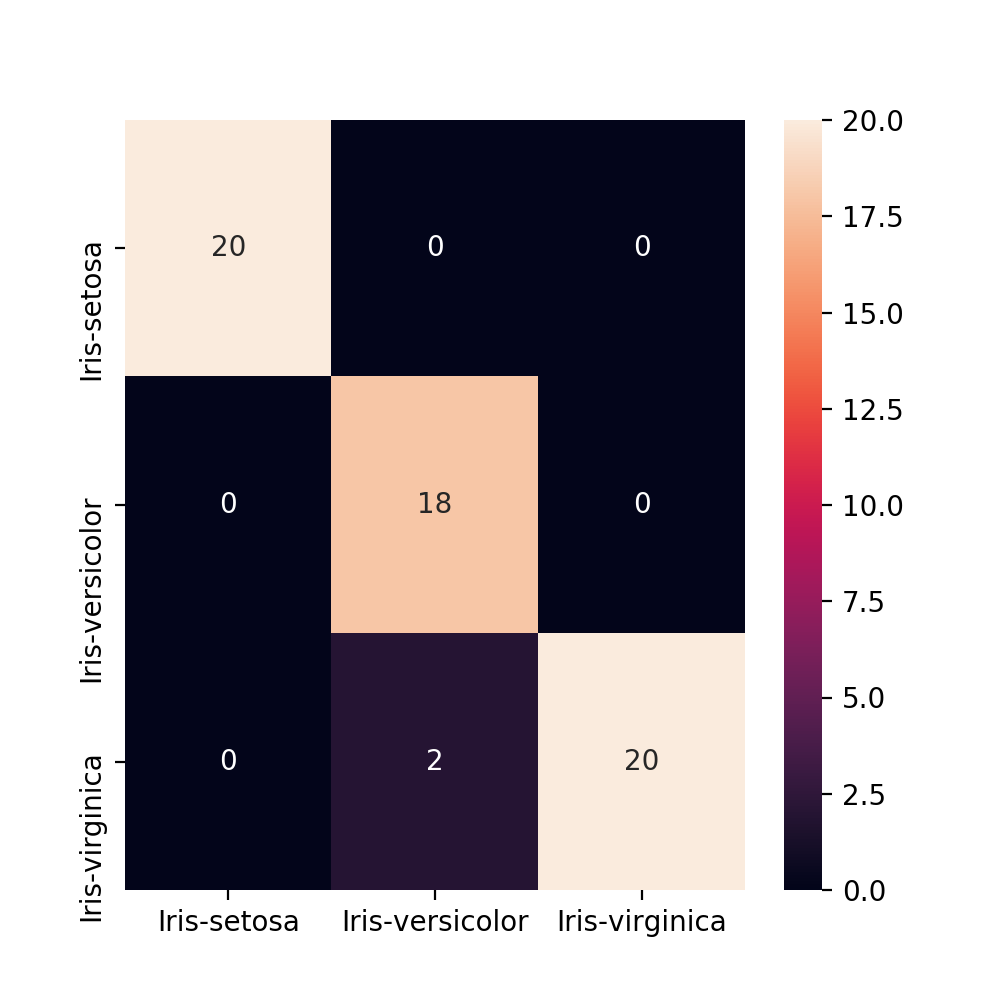
\includegraphics[width=0.45\textwidth]{../images/CM_test_no_sepal_width.png}%
      \label{fig:CM_test_no_sepal_width}%
    }\qquad
    \subfloat[Train dataset]{%
      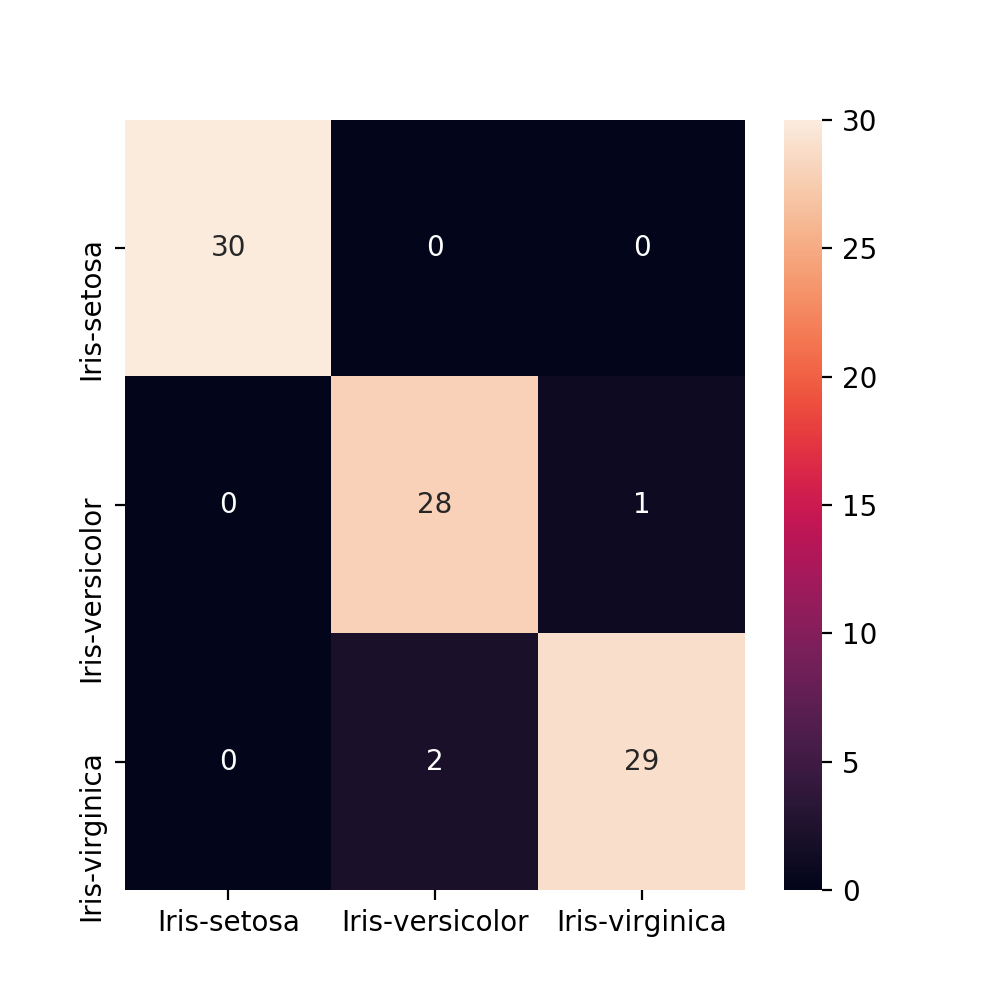
\includegraphics[width=0.45\textwidth]{../images/CM_train_no_sepal_width.png}%
      \label{fig:CM_train_no_sepal_width}%
    }
    \caption{Confusion matrices gained by using the first 30 samples as train dataset%
    and excluding the Sepal width feature;%
    $\alpha = 0.006$; 1000 iterations on $W$.}\label{fig:CM_no_sepal_width}
\end{figure}

Continuing with removing non-linear features, we also observe that there is a lot of overlap
in the Sepal length, and so this is the next feature that we want to remove. We are now left
with only the Petal width and length for our classifier to work with. The same analysis of
MSE and error rate is done for this variant of the dataset, and has been provided in
\autoref{fig:tuning_no_sepal_width_length}


\begin{figure}
    \centering
    \subfloat[MSE]{%
      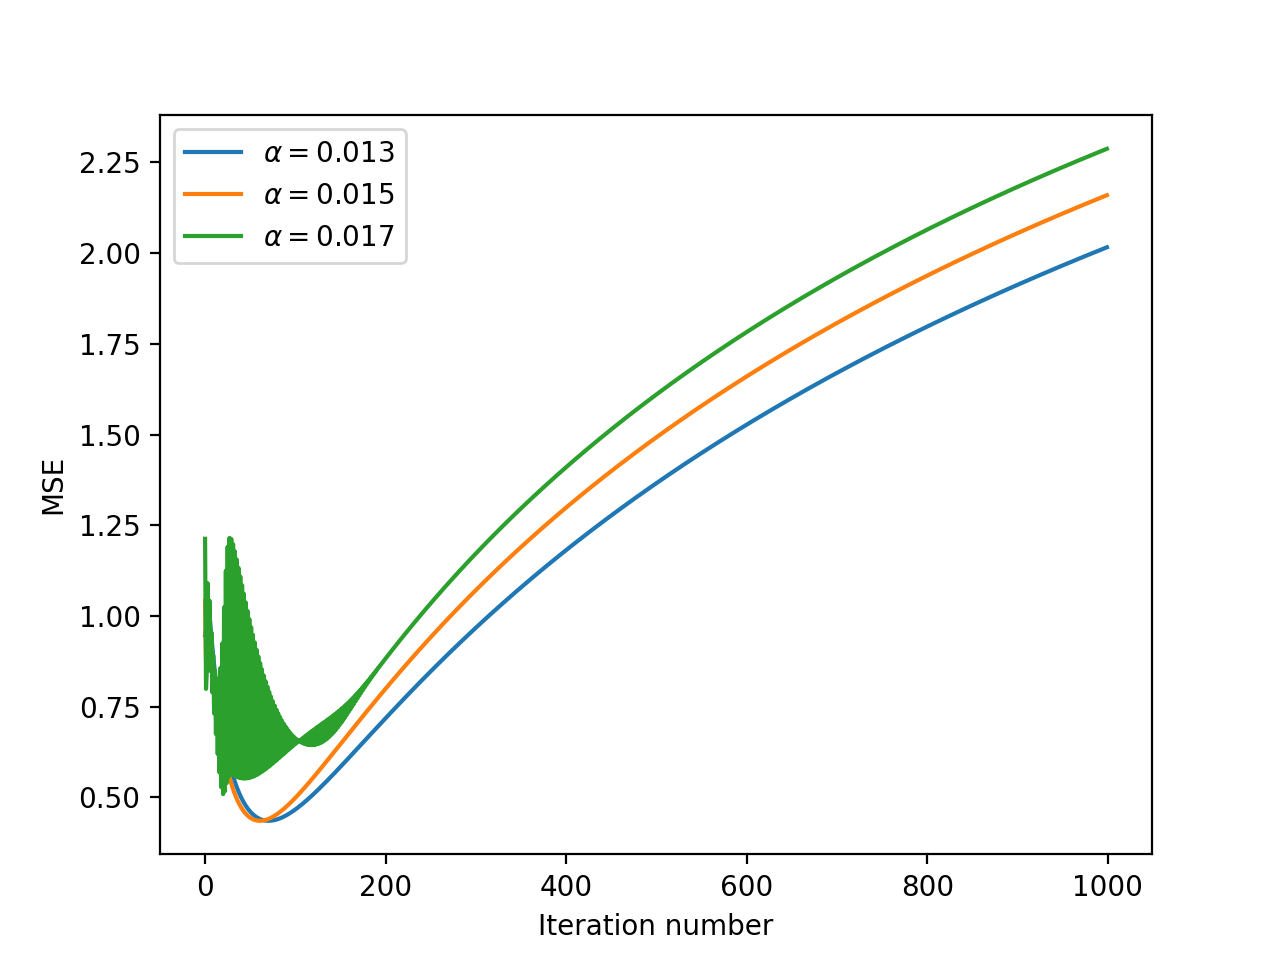
\includegraphics[width=0.55\textwidth]{../images/MSE_no_sepal_width_length.png}%
      \label{fig:MSE_no_sepal_width_length}%
    }
    \subfloat[Error rate for $\alpha=0.015$]{%
      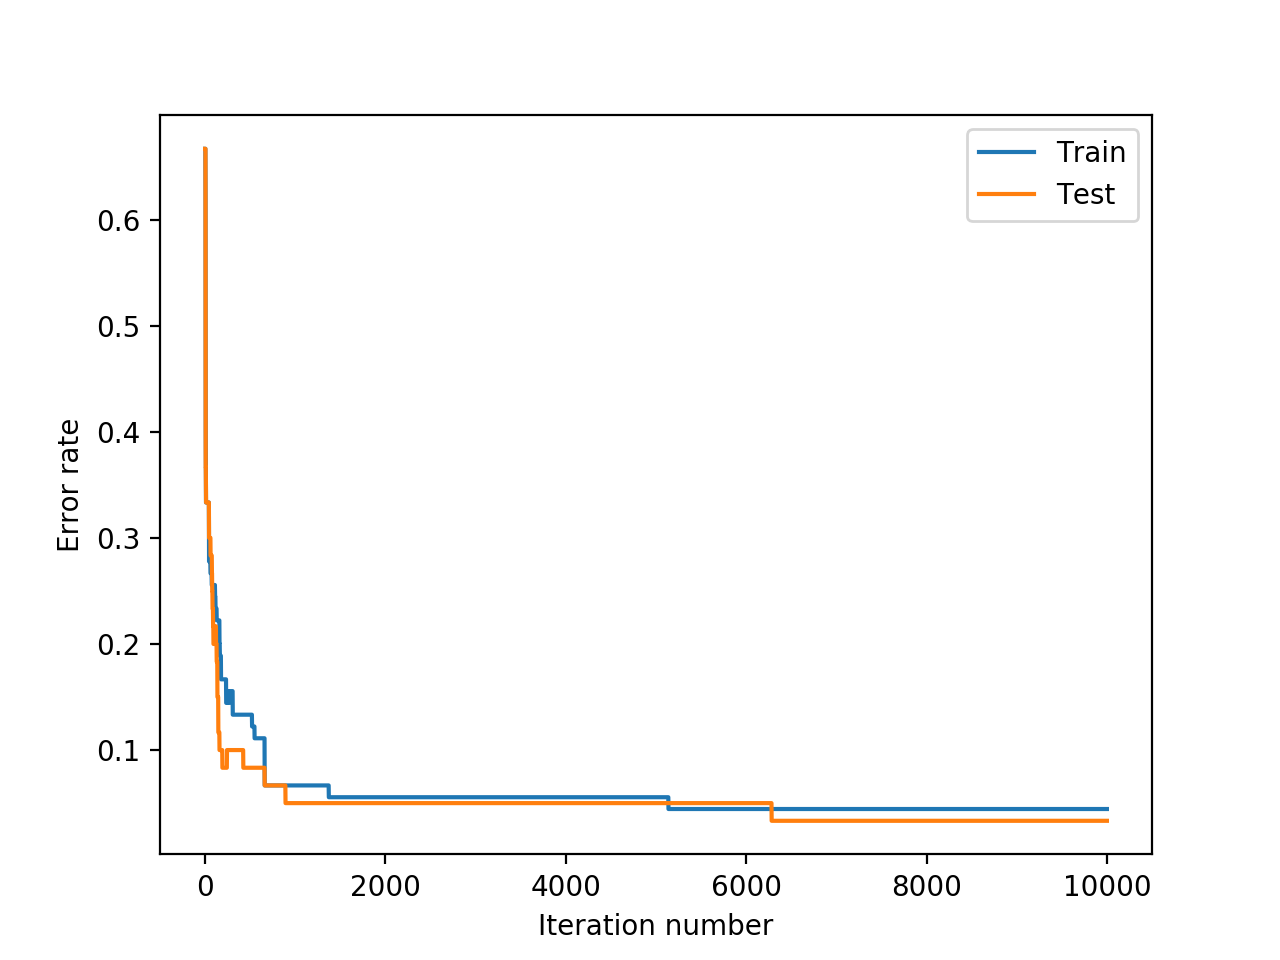
\includegraphics[width=0.45\textwidth]{../images/error_rate_no_sepal_width_length.png}%
      \label{fig:error_rate_no_sepal_width_length}%
    }
    \caption{Mean Square Error (MSE) and error rate as a function of the number of iterations on W
    for different values of $\alpha$. Using dataset without Sepal width and length.}%
    \label{fig:tuning_no_sepal_width_length}
\end{figure}

As we see, the trend we saw for the dataset without Sepal width where error rate took longer
too converge just seems to continue. We do now require a whopping 6500 iterations on our weight
matrix for it to converge. We would then expect the error rate to go down by some amount - both
since we removed overlapping features and since we used more computing power to get to it.

\begin{figure}
    \centering
    \subfloat[Test dataset]{%
      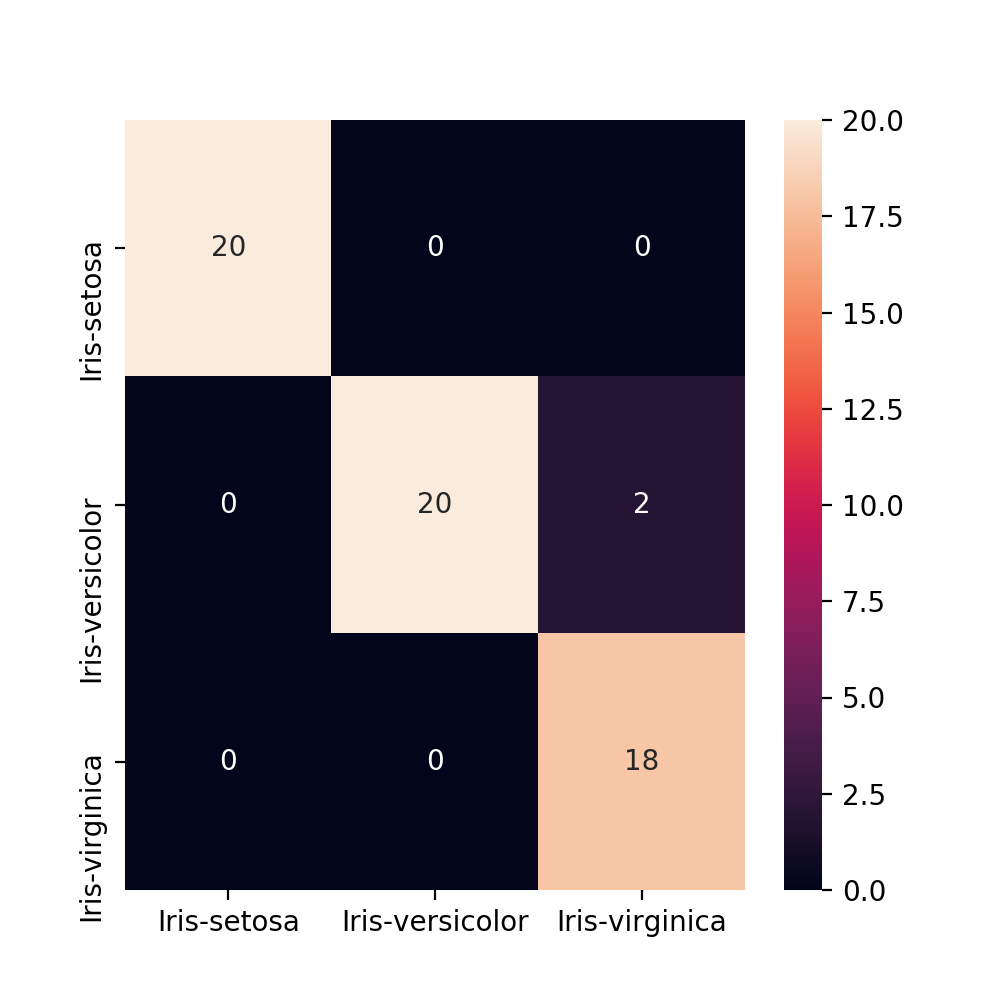
\includegraphics[width=0.45\textwidth]{../images/CM_test_no_sepal_width_length.png}%
      \label{fig:CM_test_no_sepal_width_length}%
    }\qquad
    \subfloat[Train dataset]{%
      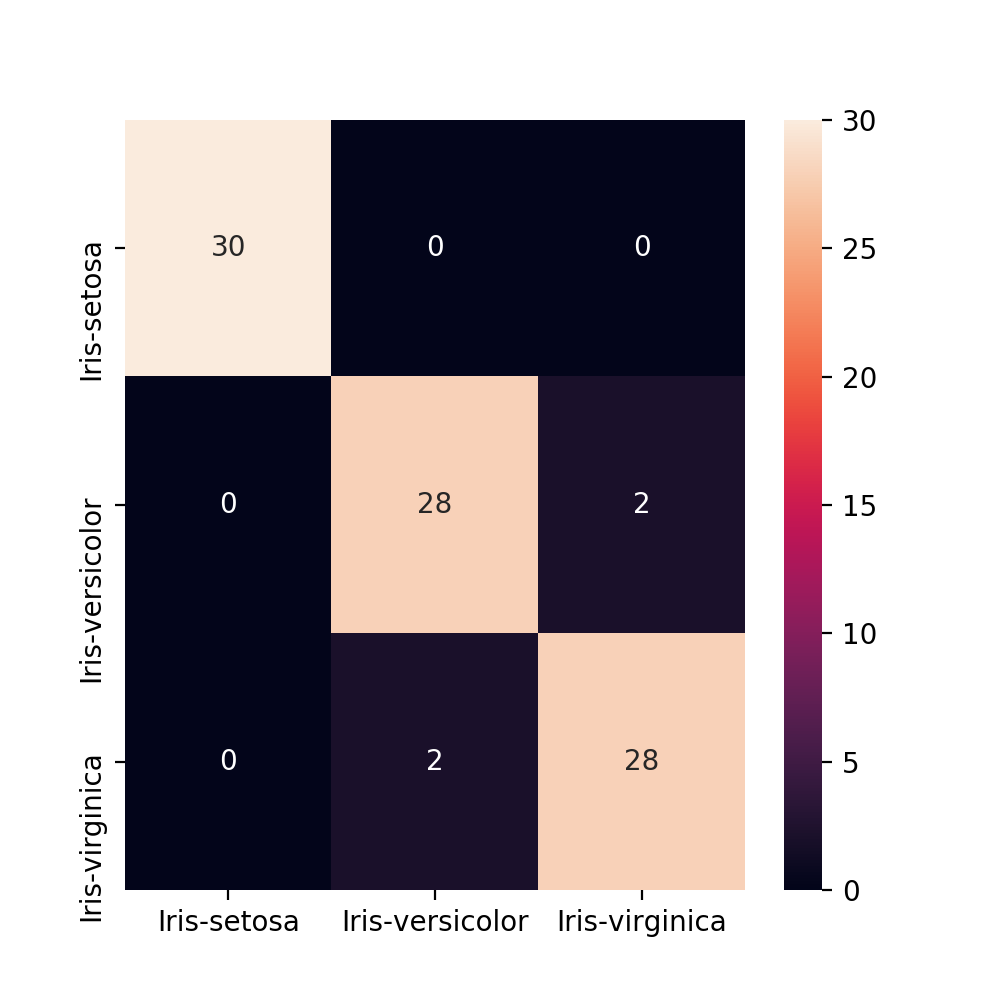
\includegraphics[width=0.45\textwidth]{../images/CM_train_no_sepal_width_length.png}%
      \label{fig:CM_train_no_sepal_width_length}%
    }
    \caption{Confusion matrices gained by using the first 30 samples as train dataset%
    and excluding the Sepal width feature;%
    $\alpha = 0.015$; 6500 iterations on $W$.}\label{fig:CM_no_sepal_width_length}
\end{figure}

However - as \autoref{fig:CM_no_sepal_width_length} reveals - this is surprisingly not the case!
We get an error rate of $3.33\%$ for the test set and $4.44\%$ for the training set.
The fact that we do not see a trend in decaying error rates makes us discard our initial assumption
that the error rate gets lower as we remove the unlinear features. Instead, we only end up having
to do more computations. And the difference in iterations is significant; While we had to do
300-400 iterations with the full feature set, we do now have to iterate 6500 times just to get
comparable results.

Just for taking it to the extremes, we continue by removing the Petal length as well, and we are
now left with only the petal width in our feature set. This leaves us with an optimal $\alpha = 0.15$
and this time we need $3000$ iterations for convergence. Neither this time we get any improvements on
error rates, with the confusion matrix being identical with \autoref{fig:CM_no_sepal_width_length}.

\section{Conclusion}

In this project, we first analyzed the impact of choosing samples for training and testing.
Here, we saw that the choice actually affected the error rate on the test set. If we were to
analyze the performance of the estimator solely on the error rate revealed by the test set, we
would have come to the wrong conclusion of saying that by using the last 30 samples for training
we actually got a  better estimator. But as we saw, both choices gave the same amount of errors
on the dataset as a whole. This leads us to draw the conclusion that it is important to choose
both a train set and a test set which are  representable for the whole population.

In the last section we studied how removing features with a lot of overlap affected the performance
of the classifier. Our initial assumption was that the classifier would perform better - after all,
a linear classifier works best on linearly separable data. However, this was not the case. We experienced
that we had to iterate the weighing matrix $W$ a lot more times just to achieve the same error rates. And
the classifier would not perform any better by further increasing the number of iterations. This makes us
draw the conclusion that removing non-linear features does not improve the performance of a linear classifier.

It should however be noted that we only had 50 samples of each feature, and so our dataset was from a
statistical point of view quite small. With only one misclassified sample give or take in difference,
it is hard to tell whether or not the classifier actually performed marginally better or if we just were
unlucky with our dataset. Also, we cannnot say on a general basis that removing non-linear features does
not improve performance; this may be the case only for samples following this exact distribution. New
research with a larger dataset, and with samples following different distributions should be conducted
in order to gain further insight into this.

\printbibliography

\end{document}